%%%%%%%%%%%%%%%%%%%%%%%%%%%%%%%%%%%%%%%%%%%%%%%%%%%%%%%%%%%%

\section{Exploring \Wikipedia{} with \WikiTax} 
\label{S:tool}

\paragraph*{\textbf{\Wikipedia's category graph}}

\Wikipedia{} uses several means of organizing its information: plain links giving rise to an article graph, designated article lists, portals meant to introduce users to key topics, infoboxes for semantic (`typed') data, and categories giving rise to a category graph for the classification of articles. When it comes to taxonomy mining, the category graph is particularly relevant; the graph is accessible, for example, through the \MediaWiki{} API\footnote{\url{http://www.mediawiki.org/wiki/API:Main_page}}, which is the access path chosen by \WikiTax.

%%%%%%%%%%%%%%%%%%%%%%%%%%%%%%%%%%%%%%%%%%%%%%%%%%%%%%%%%%%%

\paragraph*{\textbf{Graph extraction and reduction with \WikiTax}}

Initially, \WikiTax{} is pointed to a root category (level 0) for extraction. Iteratively, subcategories and pages (in fact, page titles) can be extracted level by level or exhaustively. Exhaustive extraction may take minutes our hours depending the root category. The \Wikipedia{} category graph contains many surprising edges, which easily implies inclusion of large irrelevant subgraphs. 

\WikiTax{} supports reduction of the graph both along level-by-level extraction and post extraction. Reduction involves the selection of edges exclusion. If all edges to a given category are excluded, then the corresponding category node also becomes excluded. (We node that a category may have multiple parent categories.) If reduction is applied post extraction, the exclusion is actually implemented as blacklisting. In this manner, all decisions can be easily revisited and adapted.

%%%%%%%%%%%%%%%%%%%%%%%%%%%%%%%%%%%%%%%%%%%%%%%%%%%%%%%%%%%%

\begin{figure}[t!]
\begin{center}
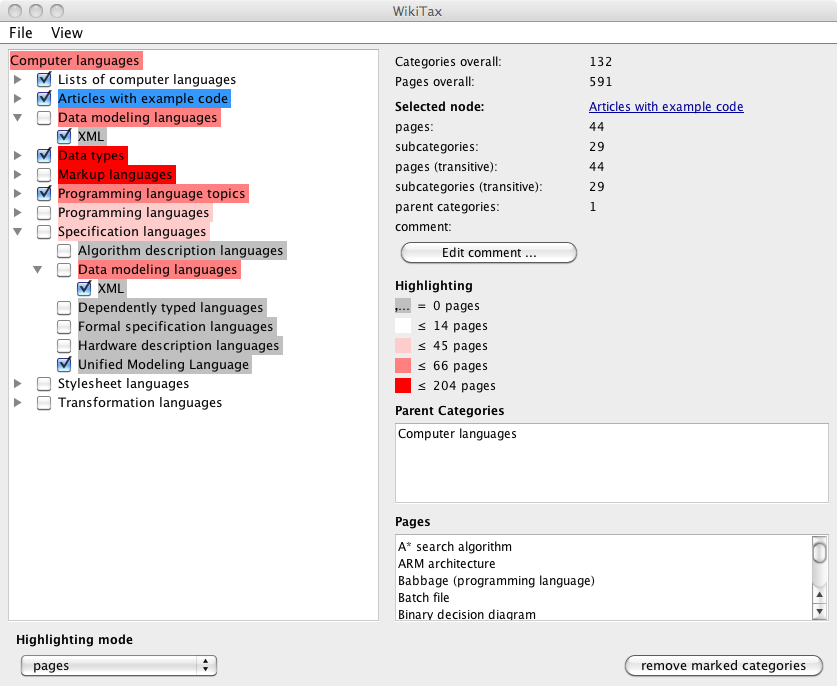
\includegraphics[width=.84\textwidth]{figures/clLevel12.png}
\end{center}
\vspace{-66\in}
\caption{Exploration of level 1 and 2 subcategories of \emph{Computer languages}.}
\label{F:clLevel12}
\vspace{-42\in}
\end{figure}

%%%%%%%%%%%%%%%%%%%%%%%%%%%%%%%%%%%%%%%%%%%%%%%%%%%%%%%%%%%%

\autoref{F:clLevel12} shows the \WikiTax{} exploration view in the following state.
Two levels (level 1 and 2) were extracted starting from the category \Wikipedia{Computer languages}. (That is, we are about to hit the `removal/blacklist' button.) Some edges are already selected for exclusion. In \S\ref{S:study}, we discuss reasons for exclusion systematically, but it suffices here to say that the selected categories are not proper language classifiers. The categories are highlighted according to the metrics of immediate member pages. We have selected the category \WikipediaCategory{Articles with example code} for which some extra data is shown in the panel on the right. All categories and pages are clickable to navigate to \Wikipedia.

%%%%%%%%%%%%%%%%%%%%%%%%%%%%%%%%%%%%%%%%%%%%%%%%%%%%%%%%%%%%

\begin{figure}[ht]
\centering
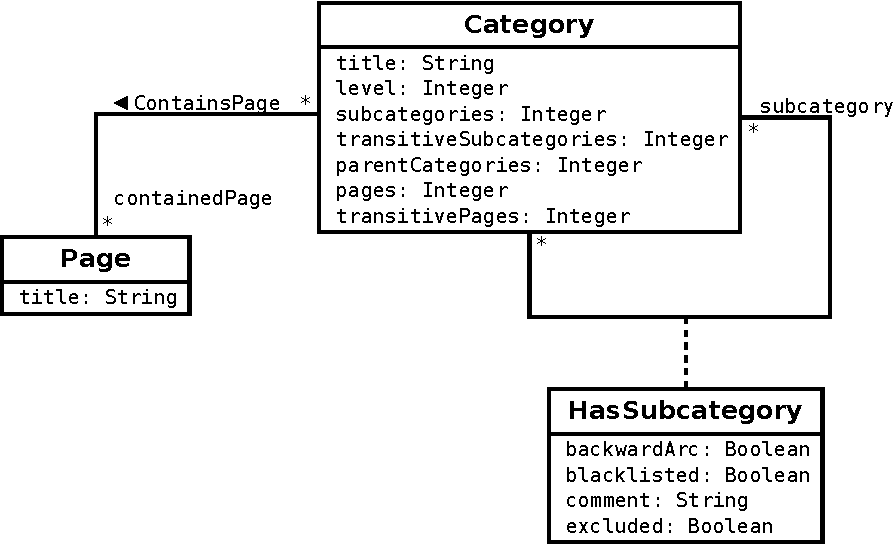
\includegraphics[width=0.63\textwidth]{../manual/figures/full_schema.pdf} 
\caption{Metamodel of the \WikiTax{} category graph.}
\label{F:metamodel}
\vspace{-42\in}
\end{figure}

%%%%%%%%%%%%%%%%%%%%%%%%%%%%%%%%%%%%%%%%%%%%%%%%%%%%%%%%%%%%

\WikiTax{} operates on an enhanced category graph; see the metamodel in \autoref{F:metamodel}. Thus, each category associates with contained pages and subcategories. The subcategory associations are attributed to keep track of metadata as follows: 

\vspace{-22\in}

{\small

\begin{description}
\item[backwardArc] Marker for cyclic edges in the category graph.
\item[blacklisted] Marker for categories blacklisted past extraction.
\item[excluded] Marker for categories excluded during reduction.
\item[comment] Label to be associated with the edge.
\end{description}

}

\vspace{-22\in}

\noindent
Categories are associated with measures as follows:

\vspace{-22\in}

{\small

\begin{description}
\item[level] The level 0, 1, 2, ... of the category in the graph with the root at level 0.
\item[subcategories] The number of immediate subcategories.
\item[transitiveSubcategories] The number of all subcategories.
\item[pages] The number of immediately contained pages.
\item[transitivePages] The number of all pages in this category.
\end{description}

}

\vspace{-22\in}

\noindent
Internally, \WikiTax{} uses the Java-based JGraLab library\footnote{\url{https://github.com/jgralab}} for the representation of (annotated) graphs with JSON as an export format. (Labels are also exposed as CSV.)

%%%%%%%%%%%%%%%%%%%%%%%%%%%%%%%%%%%%%%%%%%%%%%%%%%%%%%%%%%%%
